\documentclass[11pt,a4paper]{report}

\hfuzz=9999pt % "fix" hbox overfull
%Path relative to the .tex file containing the \includegraphics command
\usepackage{graphicx}
\usepackage{hyperref}
\hypersetup{
    colorlinks=true,
    linkcolor=blue,
    filecolor=magenta,      
    urlcolor=blue
}

\begin{titlepage}
\title{BU5526 - Portfolio Analysis \\ Lecture Notes}
\author{Rodrigo Miguel}
\date{\today}
\end{titlepage}

\begin{document}
\maketitle
\tableofcontents

\chapter{Introduction}
\section{Asset Pricing}
\subsection{Asset}
Something valuable that an entity owns, benefits from, or has use of, in generating income.
\subsection{Asset Pricing}
Needed to buy/sell at a fair price.
\begin{itemize}
    \item Obtained by discovery process:
        \begin{itemize}
            \item Demand and supply forces.
        \end{itemize}
    \item The price of an asset is simply the current value of its cash-flows.
    \[ PV = \frac{FV_1}{(1+r)^1} + \frac{FV_2}{(1+r)^2}+ ... + \frac{FV_n}{(1+r)^n} \]
        \item What we need:
        \begin{itemize}
            \item Prediction of cash flows;
            \item Discount rate.
        \end{itemize}
\end{itemize}

\subsection{How to price a stock:}
\begin{itemize}
    \item Dividend Discount Model;
    \item FCF Model;
    \item Multipliers and Comparable approach.
\end{itemize}
Being able to estimate the required \textbf{rate of return} is everything you need to calculate the \textbf{value of any asset} - once you have predicted \textbf{future cash-flows}, including:
\begin{itemize}
    \item Estimating the value of a stock;
    \item Estimating the value of a firm.
\end{itemize}

\section{Portfolio Management}
\textbf{Prudent} administration of \textbf{investable} (liquid) assets, aimed at achieving an \textbf{optimum risk-reward ratio}.

\section{Mathematical Concepts}
\subsection{Mean} An average of different observations.
\begin{itemize}
    \item Useful to describe a population;
    \item \textbf{Arithmetical}: sum of observations divided by the number of observations (if with equal weights).
    \[\overline{X} = \frac{X_1 + X_2 + ... + X_n}{n}\]
    or
    \[\overline{X} = W_1 \times X_1 + W_2 \times X_2 + ... + W_n \times X_n\]
    \item \textbf{Geometrical}: n root of the product of observations.
    \[\overline{X}_G = \sqrt[n]{X_1 \times X_2 \times ... \times X_n}\]
    or
    \[\overline{X}_G = \sqrt[1]{X_1^{W_1} \times X_2^{W_2} \times ... \times X_n^{W_n}} \]
\end{itemize}
There is a reason to use arithmetical or geometrical mean.
\begin{itemize}
    \item \textbf{Equally weighted}: when all the observations have the same importance.
    \item \textbf{Unequally weighted}: different importance for different observations.
\end{itemize}

\subsection{Variance} Seen as an extension of the mean.
\begin{itemize}
    \item Dispersion to the mean (higher/lower):
    \begin{itemize}
        \item Average of differences from the mean.
        \[\sigma_x^2 = \frac{(X_1 - \mu_X)^2 + (X_2 - \mu_X)^2 + ... + (X_n - \mu_X)^2}{n}\]
    \end{itemize}
    
\end{itemize}

\subsection{Important Statistical Concept}
\begin{itemize}
    \item The formula is correct if we possess all the data on the population;
    \item If we only have a sample, we need to reflect "impreciseness" by removing "one degree of freedom".
    \[\sigma_x^2 = \frac{(X_1 - \mu_X)^2 + (X_2 - \mu_X)^2 + ... + (X_n - \mu_X)^2}{n-1}\]
\end{itemize}
This will \textbf{always} be the case in finance.

\subsection{Standard Deviation}
\[\sigma_X = \sqrt[2]{\frac{(X_1 - \mu_n)^2 + (X_2 - \mu_n)^2 + ... + (X_n - \mu_n)^2}{(n-1)}} \]

\subsection{Skewness}
Brings back the sign. A positive skewness means more positive-value and reversely.
\[\sigma_X^3 = \frac{(X_1 - \mu_n)^3 + (X_2 - \mu_n)^3 + ... + (X_n - \mu_n)^3}{n} \]

\subsection{Kurtosis}
Outweighs extremes - dropping the sign.
\[\sigma_X^4 = \frac{(X_1 - \mu_n)^4 + (X_2 - \mu_n)^4 + ... + (X_n - \mu_n)^4}{n} \]
A large Kurtosis means a lot of extreme values.
\begin{itemize}
    \item To get a \textbf{meaningful estimate:} \textbf{excess} kurtosis needs to be provided.
    \item Kurtosis of a normal distribution is 3.
\end{itemize}

\paragraph{Note:} Unbiased equations of these two indicators are slightly more complex, but computer packages provide them automatically.

\section{Assumptions of Mean-Variance Analysis}
\begin{itemize}
    \item Allows describing different assets simply.
    \item Assumes returns are normally distributed.
\end{itemize}
\subsection{Normal distribution}
\begin{itemize}
    \item Its mean and median are equal;
    \item It's defined by two parameters, mean and variance;
    \item It's defined around its mean with:
    \begin{itemize}
        \item 68\% of observations within $\pm$ 1$\sigma$ of the mean.
        \item 95\% of observations within $\pm$ 2$\sigma$ of the mean.
        \item 99\% of observations within $\pm$ 3$\sigma$ of the mean
    \end{itemize}
    \item Returns are not normally distributed.
    \begin{itemize}
        \item Skewed: not symmetric around the mean.
        \item Characterized by high probability of extreme event.
    \end{itemize}
\end{itemize}

\section{Returns on Financial Assets}
\subsection{Holding period return} Return from holding an asset for a specific period of time.
\[R = \frac{P_t - P_{t-1}}{P_{t-1}} + \frac{D_t}{P_{t-1}}\]
Capital gain + Dividend yield \\
Holding period returns = compound returns
\[R = [(1 + r_1) \times (1 + r_2) \times (1+r_3)] - 1 \]

\subsection{Geometric Mean Return}
\[\overline{R} = \sqrt[T]{(1+r_{i_1}) \times (1+r_{i_2}) \times ... \times (1+r_{i_T})} - 1\]
\subsection{Annualized Return} These returns should be capitalized.
\begin{itemize}
    \item Such as:
    \[ r_{annual} = (1+r_{period})^C - 1\] with C being the number of periods in a year.
\end{itemize}

\subsection{Portfolio Return}
\begin{itemize}
    \item When several assets are combined into a portfolio, we can compute the portfolio return.
    \item Weighted average of the returns of individual assets
    \[ R_p = W_1 \times R_1 + W_2 \times R_2\]
\end{itemize}

\subsection{Historical and Expected Returns}
\begin{itemize}
    \item Computed from historical data.
    \item What the investor expects to earn.
    \item Historical returns are different from expected returns.
\end{itemize}

\subsection{Ways of Calculating Expected Returns}
\begin{itemize}
    \item Gut feeling;
    \item Modelling - calculated from a formula.
\end{itemize}

\subsection{Standard deviation - Volatility}
\begin{itemize}
    \item Historical standard deviation;
    \item Defined as \textbf{risk} of equity return.
\end{itemize}

\subsection{Portfolio Variance}
\begin{itemize}
    \item Cannot simply add up two variances.
    \item Covariance:
    \[cov(X,Y) = E(XY) - E(X) \times E(Y)\]
    \begin{itemize}
        \item The more the two assets move in the same way, the higher the covariance.
        \item A negative covariance means the assets move in opposite directions.
    \end{itemize}
    \item Variance:
    \[ \sigma_v^2 = wCw^T \]
\end{itemize}

\subsection{Correlation and Portfolio Risk}
The correlation among assets determine the portfolio's risk.
\begin{itemize}
    \item Is a measure of tendency for N investments to act similarly;
    \item Can range from $-$1 and $+$1.
    \[\rho_{ij} = \frac{cov(R_i,R_j)}{\sigma_i \sigma_j}\]
\end{itemize}

\chapter{The Optimal Portfolio}
\section{Portfolio}
\subsection{The Portfolio Perspective on Investing}
One of the biggest challenges faced by individuals and institutions is to decide on how to invest for future needs. Should they invest in individual securities, or should they take a portfolio approach?
\\A portfolio and evaluating individual securities in relation to their contribution to the investment characteristics is important to achieve a "good" and "safe" return.
\subsection{Diversification: Avoiding Disaster}
Portfolio diversification helps investors avoiding disasters. It is of our utmost priority to balance investment weights as a way of having a good risk-return ratio.
\\On the other hand, it does not mean that, by reducing risk the portfolio will have reduced profits.
\begin{itemize}
    \item The portfolio approach provides investors with \underline{a way to reduce the risk} associated with their investment.
    \item Investors can choose the risk-return trade-off they prefer.
    \item A lower risk does not necessarily mean lower profits.
\end{itemize}
\subsection{Reducing Risk}
A Portfolio generally offers equivalent expected returns with lower overall volatility.
\\How to calculate its standard deviation?
\begin{itemize}
    \item An interesting feature of combining assets is that:
    \item \begin{itemize}
        \item While the combined return is the weighted average of individual returns, the combined variance is impacted by the covariance between securities.
    \end{itemize}
    \item{Covariance is how securities move together.}
\end{itemize}
\subsubsection{Variance of a Portfolio}
\[\sigma_p{^2} = wCw^T\]
or
\[\sigma_v{^2} = w_1{^2}\sigma_1{^2} + w_2{^2}\sigma_2{^2} + 2w_1w_2c_{12}\]

Remember that using correlation instead of variance, we can reformulate the variance equation:
\[\sigma_v{^2} = w_1{^2}\sigma_1{^2} + w_2{^2}\sigma_2{^2} + 2w_1w_2\sigma_1\sigma_2\rho_{12}\]

This equation shows that as long as $\rho_{12} is < 1$ adding more assets will reduce the overall variance of the portfolio.

\subsubsection{Standard Deviation}
\[\sigma_p = \sqrt{\sigma_p{^2}}\]

\subsection{Correlation and Portfolio Risk}
\begin{itemize}
    \item A major reason that portfolios can effectively reduce risk is that combining securities whose returns do not move together provides diversification.
    \item The less correlated the assets, the better the risk-return trade-off obtained within a portfolio.
\end{itemize}

\subsection{Return and Risk of a Portfolio}
\begin{itemize}
    \item This is the fundamental idea of \textbf{diversification};
    \item Because assets do not move perfectly together (correlation $= 1$), combining several assets will reduce the overall variance;
    \item Assets don't need to be negatively correlated, just not perfectly correlated (correlation $< 1$)
    \item The more uncorrelated the assets, the greater the risk-return trade-off.
\end{itemize}
\subsection{Avenues for Diversification}
\begin{itemize}
    \item Diversify with asset classes;
    \item Diversify with index funds;
    \item Diversify among countries;
    \item Buy insurance;
    \item Buy put options;
    \item Evaluate the assets.
\end{itemize}

\subsection{Diversification: Not necessarily Downside Protection}
\begin{itemize}
    \item It does not mean that diversification eliminates the entire risk.
    \item It removes only unsystematic (idiosyncratic) risk.
    \\ Total Risk = Systematic Risk + Unsystematic Risk
\end{itemize}
\begin{figure}[h]
    \centering
    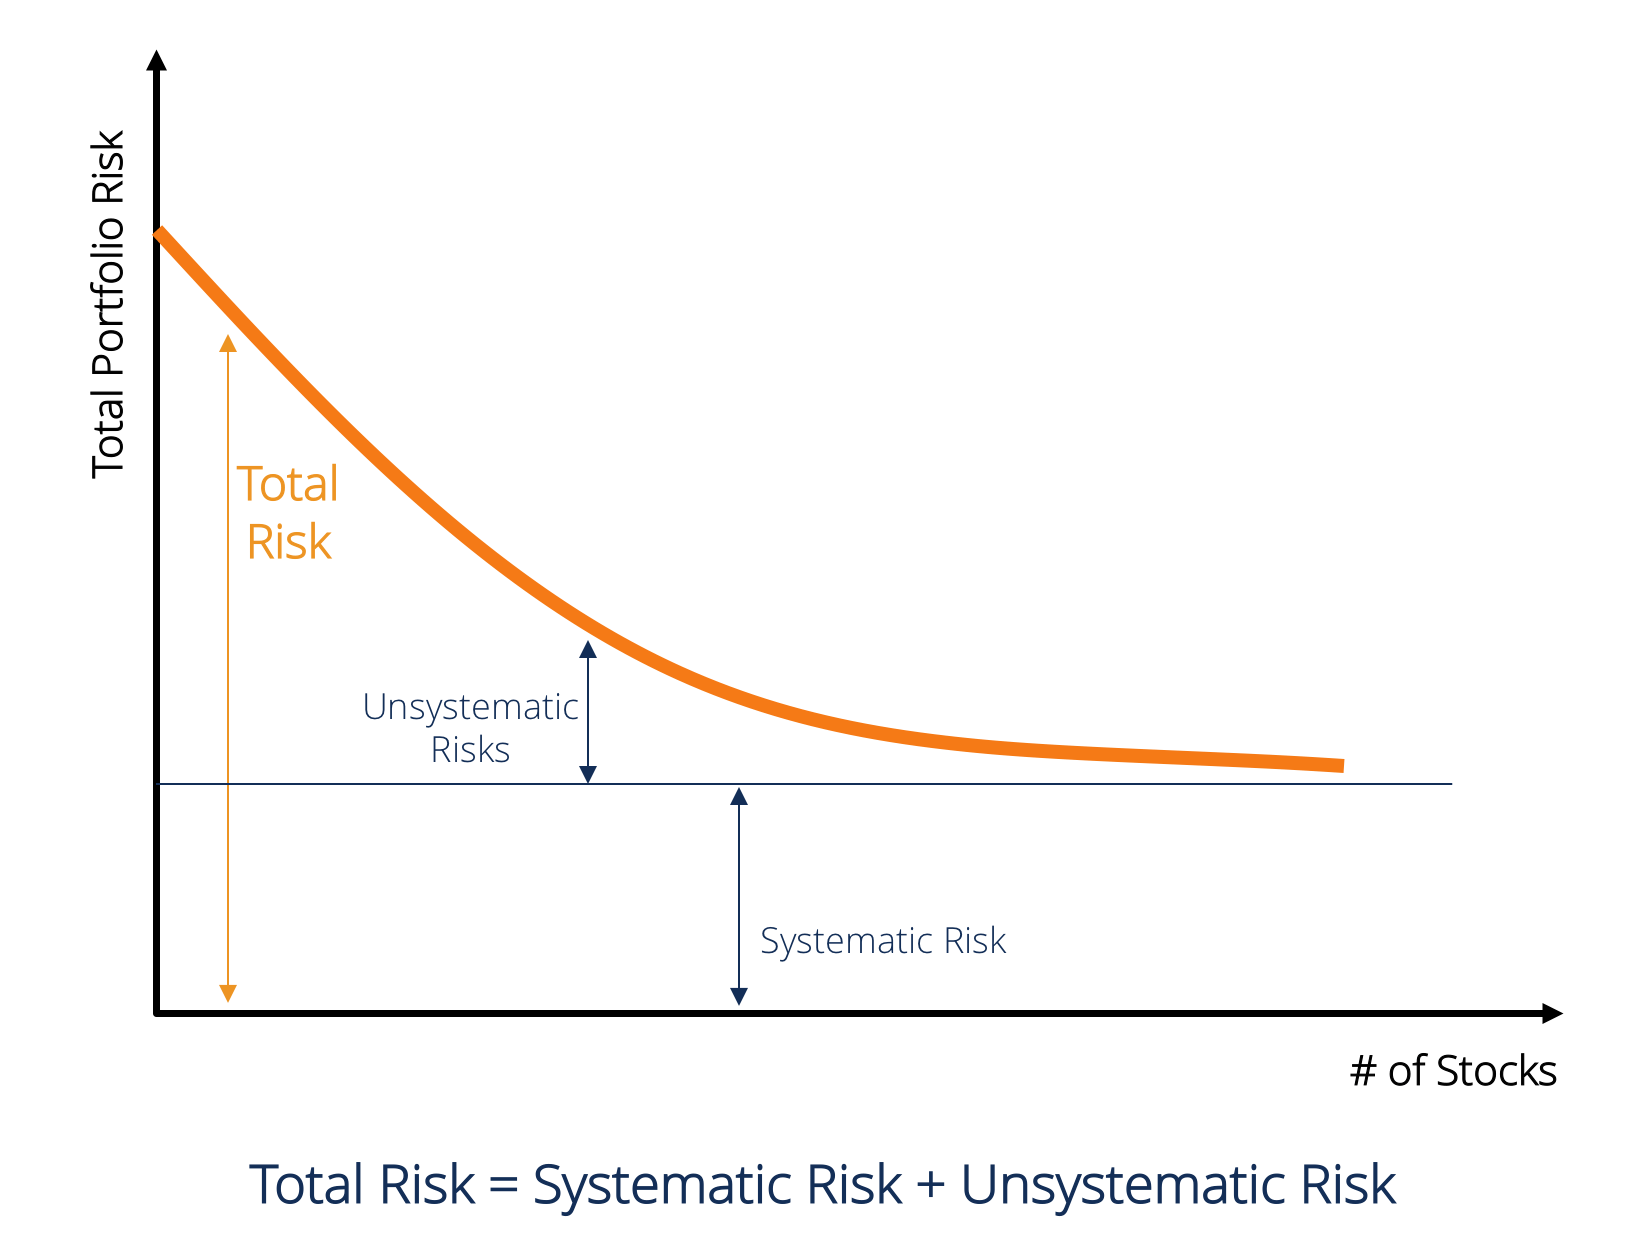
\includegraphics[width=\textwidth]{images/totalrisk.png}
\end{figure}

\paragraph{Unsystematic Risk} Is the risk specific to a company or industry. It is also known as diversifiable risk. It can be reduced through diversification.
\paragraph{Systematic Risk} Is the risk specific to the entire market. Also known as undiversifiable risk, affecting the overall market.


\begin{itemize}
    \item The benefit of diversification varies over time.
    \begin{itemize}
        \item Correlation among assets might change;
        \item Diversification does not protect against a generalized decrease in returns and increase in risk.
    \end{itemize}
    \item When all assets move together, like during a financial crisis, diversification benefits shrink.
    \begin{itemize}
        \item Hedging against risk becomes more difficult.
    \end{itemize}
\end{itemize}

\subsection{The Emergence of Modern Portfolio Theory}
\begin{itemize}
    \item The concept and intuition of the benefit of diversification has been around for a long time.
    \item However, its modern concept is theorized more recently.
    \item The main conclusion is that: \textbf{investors should not only hold portfolios but also focus on the correlation among the securities included.}
\end{itemize}

\section{Efficient Portfolio Frontier}
\subsection{Investment Opportunity Set}
Include as many assets as possible, from different sectors.
\subsection{Minimum Variance Frontier}
\begin{itemize} 
    \item We create a portfolio of assets;
    \item We are interested in pushing the frontier onto the north-west: 
    \begin{itemize}
        \item Minimizing the variance for a given return.
    \end{itemize}
    \item We calculate the combinations with different weights that minimize the variance for a given return.
    \item If we combine all the available assets and select the weights giving the lower variance for a given return, we end up with the \textbf{minimum variance frontier}.
    \item All portfolios on this frontier display a lower variance and a higher return than any individual asset.
\end{itemize}
\paragraph{Note:} The frontier uses all the available assets.
An efficient portfolio is \textit{any} portfolio on the minimum variance frontier.

\section{The Efficient Portfolio}
\subsection{Risk-free Asset}
\begin{itemize}
    \item To select the most efficient portfolio on the frontier, we need to add a risk-free asset.
    \item A risk-free asset will allow us to:
    \begin{itemize}
        \item Find the most efficient portfolio;
        \item Draw the capital allocation line (CAL);
        \item Create any risk-return combination for investors.
    \end{itemize}
    \item The efficient \textbf{investor portfolio} will always be a \textbf{combination} of:
    \begin{itemize}
        \item The risk-free asset;
        \item The efficient portfolio.
    \end{itemize}
\end{itemize}

\section{Capital Allocation Line}
\begin{itemize}
    \item A capital allocation line is a line that allocates capital between two assets;
    \item We will allocate between a risk-free and a risky asset;
    \item We will still think in terms of risk and return trade-off;
    \item We need two elements: an \textbf{intercept}, and a \textbf{slope}.
\end{itemize}
\subsection{A Risk-free Asset}
In our case, assume a portfolio of two assets, a risk-free asset and a risky asset. Expected return can be determined as:
\[E(R_p) = W_1R_f + (1-W_1)E(R_i)\]
Because the risk-free asset has 0 risk, its variance is equal to zero, hence, the variance of this portfolio can be calculated as:
\[\sigma_p{^2} = (1-W_1)^2\sigma_i{^2}\]
And volatility:
\[\sigma_p = \sqrt{(1-W_1)^2\sigma_i{^2}} = (1-W_1)\sigma_i \]
If we combine the portfolio return and standard deviation formula, we can rewrite the expected return in terms of risk.
\\ The expected return of a portfolio that mixes a risk-free asset and the optimal portfolio is based on two elements:
\[E[R_p] = R_f + \frac{E(R_i) - R_f}{\sigma_i}\sigma_i\]
\begin{itemize}
    \item The risk-free rate: $R_f$
    \begin{itemize}
        \item It is the Y-intercept;
        \item You cannot earn less than that.
    \end{itemize}
    \item The market price of risk: $\frac{E(R_i)-R_f}{\sigma_i}\sigma_p$
    \begin{itemize}
        \item It is the slope of the capital allocation line (CAL);
        \item The highest, the best: plus it is high, plus the risk is profitable.
    \end{itemize}
\end{itemize}
\subsection{The Capital Allocation Line (CAL)}
\begin{itemize}
    \item The combination between a risky asset and a risk-free asset is called the \textbf{capital allocation line};
    \item The risk-free rate does not change;
    \item Maximizing this angle maximizes your benefits for the risk you are taking.
    \item You do not control the market price of risk;
    \begin{itemize}
        \item It is priced by the market.
    \end{itemize}
    \item At an investor level, you can vary your risk, by changing your weights in the portfolio.
\end{itemize}
\subsection{CAL and Optimal Portfolio}
\begin{itemize}
    \item Using the CAL, we will now find \textbf{the} optimal portfolio;
    \item It is one of the portfolios on the efficient frontier;
    \item By using the risk-free asset, you maximize your risk-return ration.
    \item Mathematically, it is the point that is tangent between the efficient frontier and the CAL.
    \item You cannot achieve a point better than one on the CAL;
    \begin{itemize}
        \item This would only be by changing the set of assets.
    \end{itemize}
    \item By holding a risk-free asset, an investor can achieve a point of higher return than the Markowitz Efficient Frontier with the same risk-level.
    \begin{itemize}
        \item Negative weight on the risk-free asset (Y).
    \end{itemize}
    \item The CAL and the optimum portfolio evolve over time.
    \begin{itemize}
        \item If the risk-free asset return changes, it will affect the CAL Y-intercept;
        \item Hence, it will modify the CAL, and which portfolio is optimum.
    \end{itemize}
\end{itemize}
\begin{figure}[h]
    \centering
    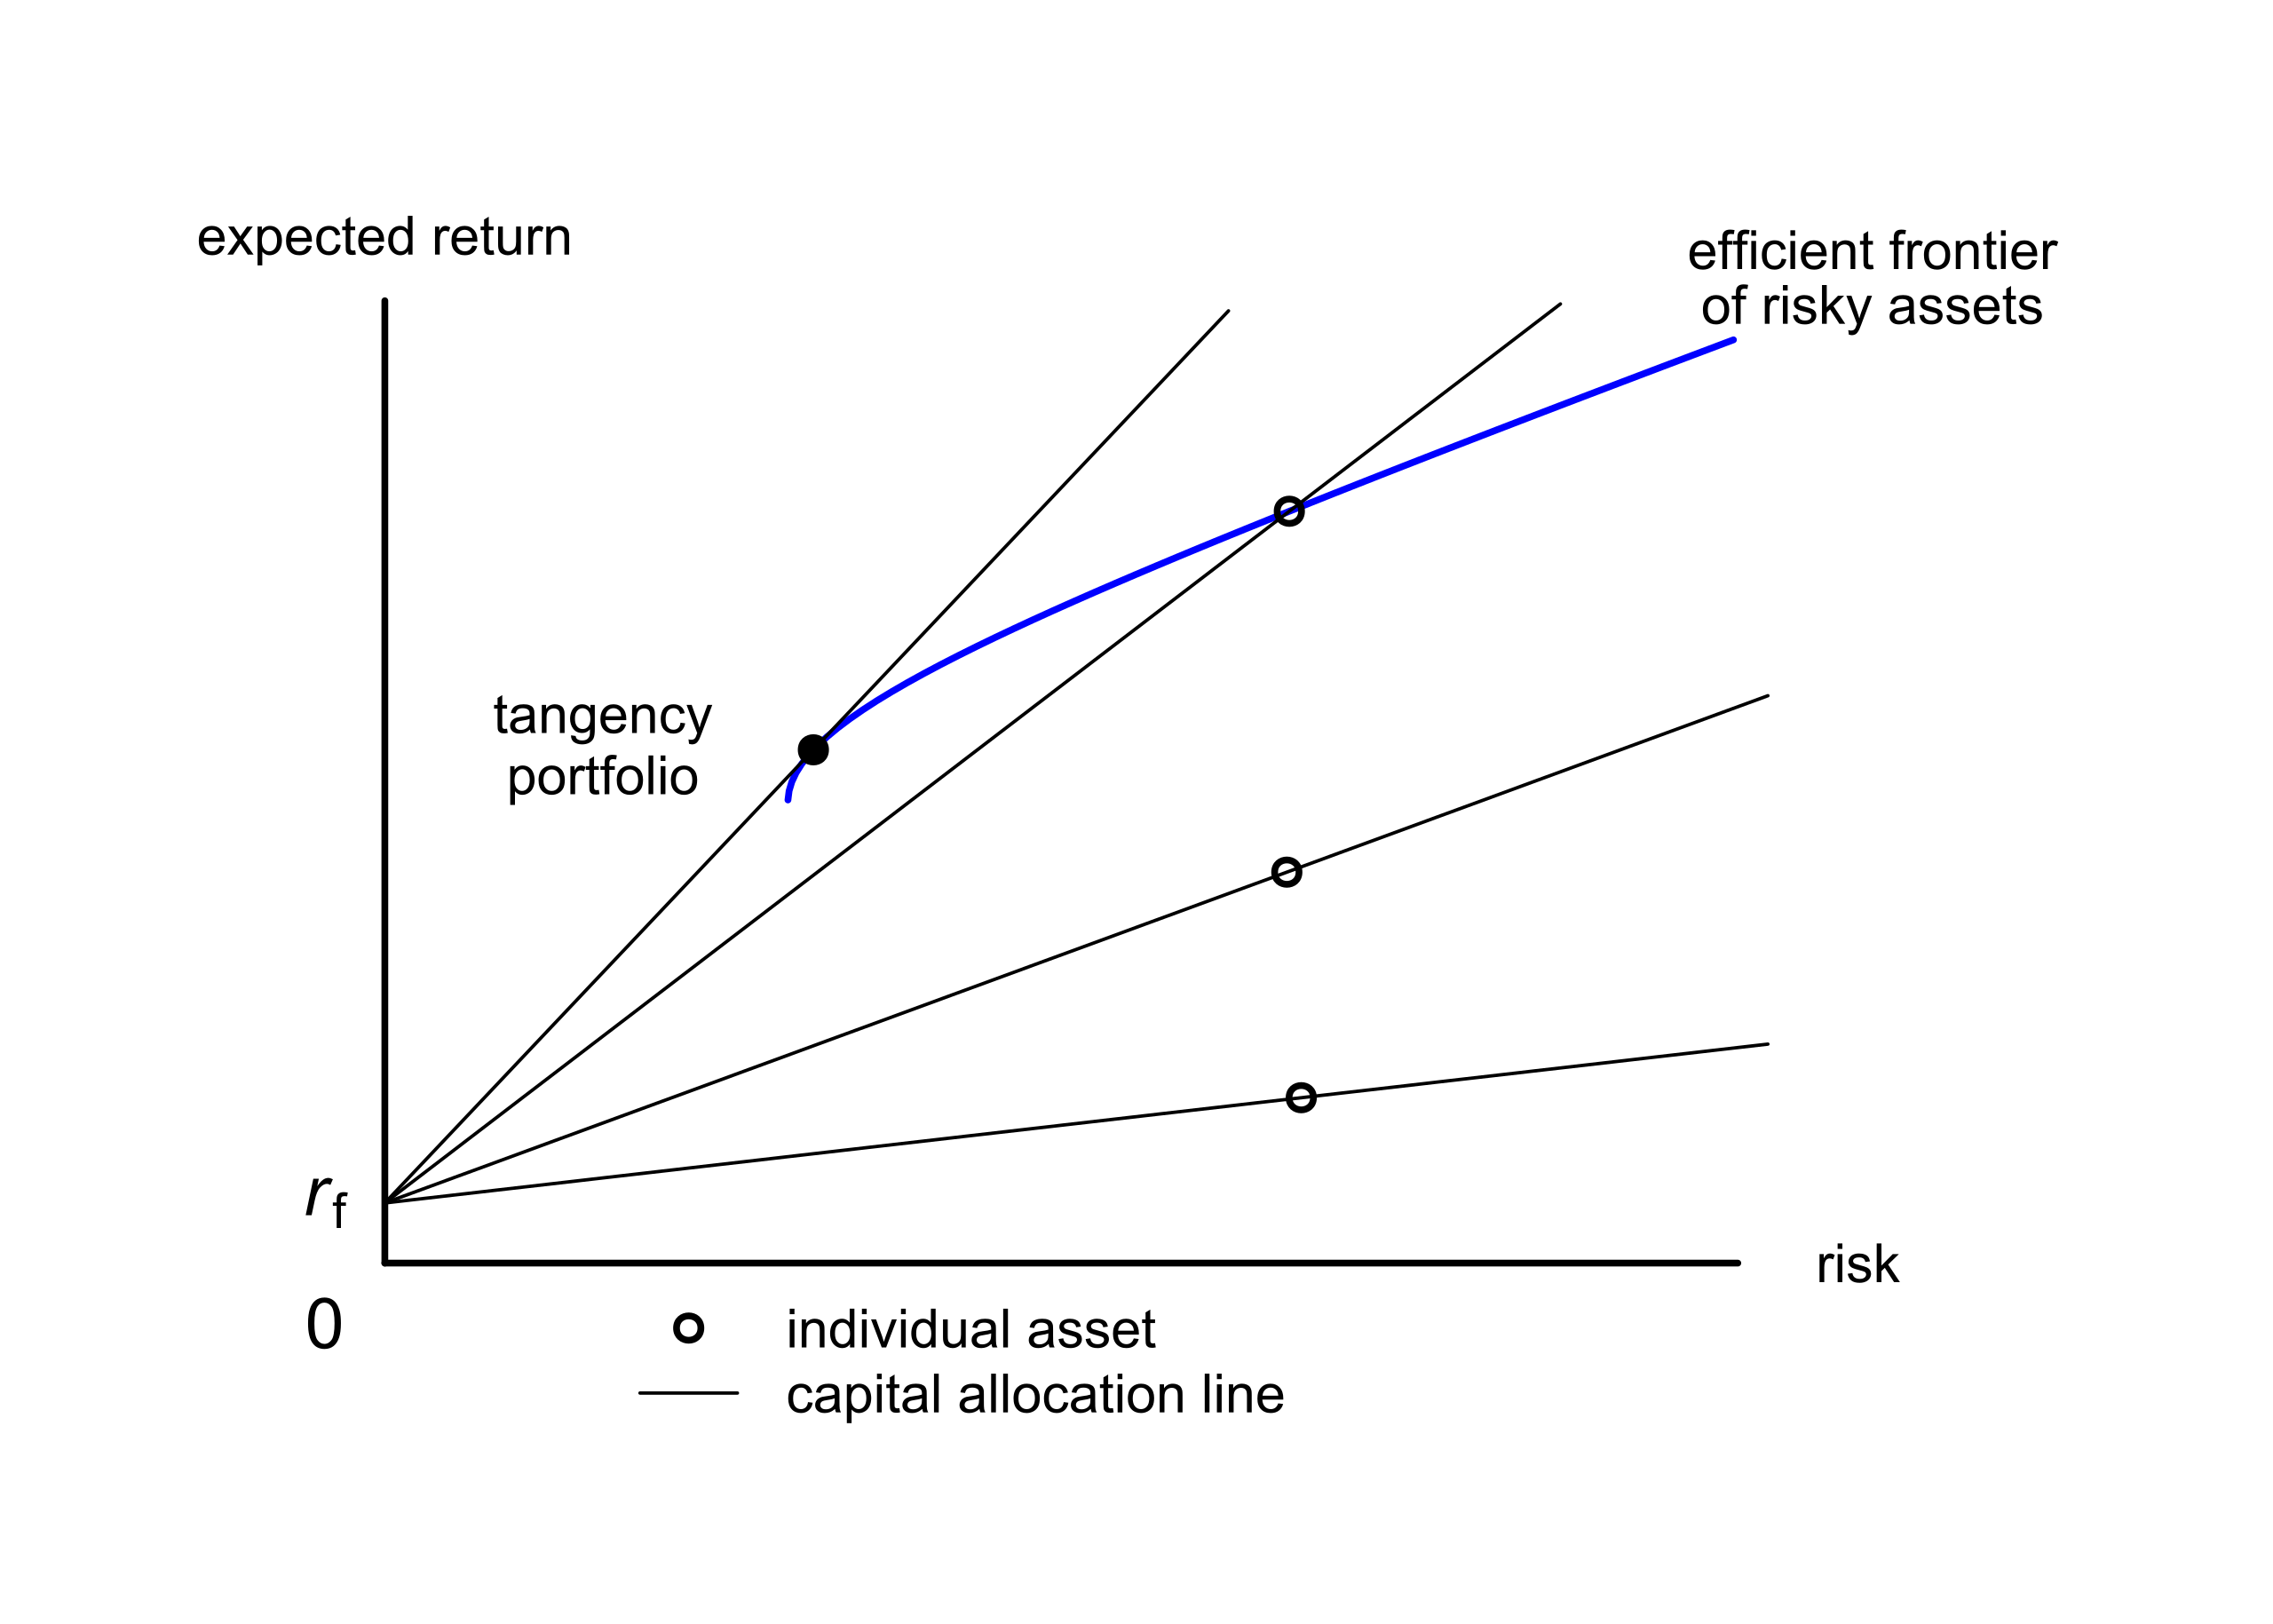
\includegraphics[width=\textwidth]{images/cap.png}
\end{figure}

\section{Optimal Investor Portfolio}
All investors will choose a \textbf{combination} of the risk-free and optimum portfolio. They will just change their weightings. But how do we know which portfolio will be chosen by a \textbf{specific investor}?
\subsection{The concept of Risk Aversion}
The choice of portfolio will differ across individuals because each individual has a different risk aversion.
\begin{itemize}
    \item Risk-seeking: utility increase with uncertainty.
    \begin{itemize}
        \item The individual will preferred a gamble with an expected value of £45 than a certain £50;
        \item Lottery and casinos.
    \end{itemize}
    \item Risk-neutral
    \begin{itemize}
        \item The individual is indifferent between the gamble or a £50 guaranteed income;
        \item A billionaire may be indifferent in this case.
    \end{itemize}
    \item Risk-adverse
    \begin{itemize}
        \item The investor will prefer a certain value of £50 than an expected value of £45;
        \item The risk-return trade-off is an indicator of risk-aversion;
        \item Historical data supports risk-aversion: higher returns, come with higher risks.
    \end{itemize}
\end{itemize}

\subsection{Utility Theory}
\begin{itemize}
    \item The \textbf{utility} he derives from the guaranteed income of £50 greater than the \textbf{utility} he derives from the alternative.
    \item Individuals are different in their preferences.
    \begin{itemize}
        \item All risk-averse investors will not rank their investments in the same manner;
        \item With a guaranteed outcome of £40, some may find it inadequate.
    \end{itemize}
    \item We can calculate the utility of an investor.
    \item This is not its return: it combines return and risk.
    \begin{itemize}
        \item Utility is a function of return for each individual;
        \item Individuals prefer higher utility.
    \end{itemize}
    \item We usually assume that investors are adverse to risk.
    \item There are plenty of ways to \textbf{modelize} utility.
\end{itemize}
\paragraph{The formula} \[U = E(r) - \frac{1}{2}A\sigma^2\]
\begin{itemize}
    \item U = Utility of an investment;
    \item E(r) = Expected Return;
    \item A = Measure of risk tolerance or risk aversion - can be either negative or positive;
    \begin{itemize}
        \item Risk adverse investor: $A>0$
        \item Risk neutral investor: $A=0$
        \item Risk seeking investor: $A<0$
    \end{itemize}
    \item $\sigma^2$ = Variance or risk.
    \item Higher returns = higher utility;
    \item Higher variance reduce/increase the utility, depending on A;
    \item A risk-free asset generates the same utility for all individuals.
\end{itemize}

\section{Indifference Curve}
An indifference curve plots the combination of risk-return pairs that an investor would accept to maintain a given level of utility. For each investor there is an infinity of indifference curves, but each indifference curve for each investor never cross over each other.
\begin{itemize}
    \item Represent the trade-off between risk and returns, with the \textit{same utility}.
    \item All risk-adverse investors will prefer curves on the north-west.
    \item Risk-adverse curves are convex because as risk increases, an investor needs even higher returns to compensate.
    \item The \textbf{slope} of curves is the \textbf{same for one investor} and different among investors.
\end{itemize}
\begin{figure}[h]
    \centering
    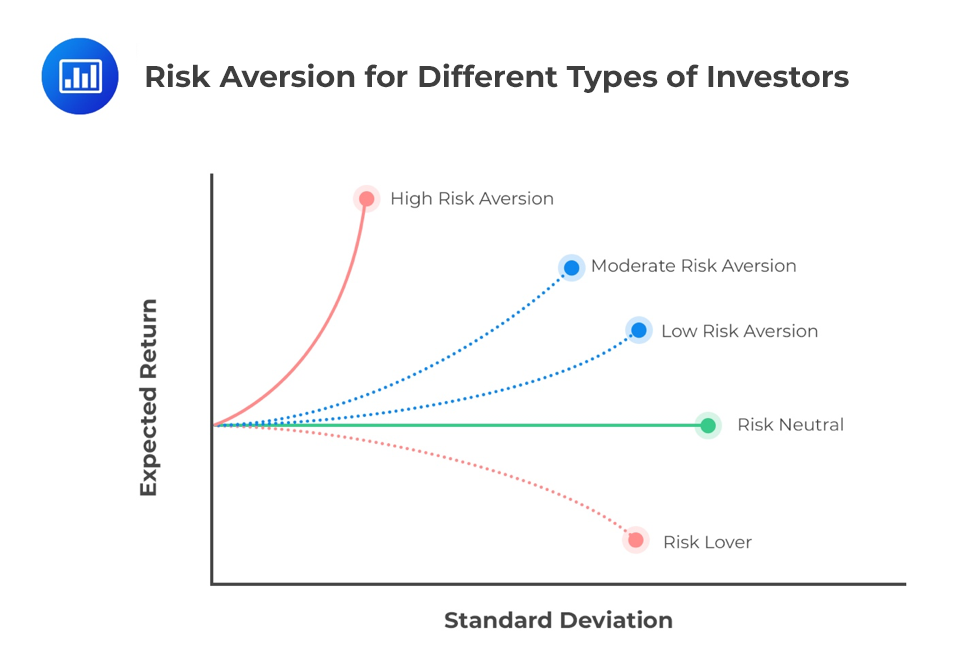
\includegraphics[width=\textwidth]{images/Risk-Aversion-for-Different-Types-of-Investors.png}
\end{figure}

\section{Optimal Investor Portfolio}
\begin{itemize}
    \item To know which combination is optimal for a given investor, we will use its indifference curve.
    \item The optimal investor's portfolio is the one which is tangent with the indifference curve.
    \begin{itemize}
        \item It gives them the highest \textbf{achievable} return.
        \item Lower or higher curbs, respectively, give:
        \begin{itemize}
            \item A lower utility;
            \item An unachievable utility.
        \end{itemize}
    \end{itemize}
    \item There is a different optimal portfolio for each investor - depending on its risk-aversion.
    \begin{itemize}
        \item All the points on CAL(P) are achievable;
        \item The selection will depend on the investor's preference.
    \end{itemize}
\end{itemize}
\section{The Two-Fund Separation Theorem}
\begin{itemize}
    \item Efficient Frontier;
    \item The Capital Allocation Line;
    \item Indifference Curve;
\end{itemize}
These concepts can be synthesized as a key theorem of modern portfolio theory.
\begin{itemize}
    \item \textbf{The two-fund separation theorem:} we can divide an investor's problem into two distinct steps.
    \begin{itemize}
        \item The investment decision;
        \item The financing decision.
    \end{itemize}
    \item \underline{For the investment decision:} all investors, regardless of taste, risk preferences and initial wealth, will hold a combination of two funds:
    \begin{itemize}
        \item A risk-free asset;
        \item The optimal portfolio of risky assets.
    \end{itemize}
    \item \textbf{Note:} All investors should lie on CAL(P).
    \item \underbar{For the financing decision:} each investor chooses the appropriate weight of risk-free and risky portfolio (P).
    \item The utility indifference curve of each investor will determine the investor's allocation to risky assets.
    \begin{itemize}
        \item Portfolios before the optimal risky portfolio are obtained by lending at the risk-free rate.
        \item Portfolios beyond the optimal risky portfolio are obtained by borrowing at the risk-free rate.
    \end{itemize}
\end{itemize}
\section{Summary of the Optimal Portfolio Choice}
\begin{itemize}
    \item Build the minimum variance frontier using all the assets available;
    \item Calculate and draw the capital allocation line (P) that is tangent to the minimum variance frontier.
    \item Use the investor's utility curves to obtain the portfolio that lies on the utility curve and on the capital allocation line (P).
\end{itemize}
\chapter{Capital Asset Pricing Model}
\section{The Capital Asset Pricing Model}
\begin{itemize}
    \item In the previous lectures, we demonstrated the diversification effect and the two-fund theorem;
    \item We know that all investors should possess the optimal portfolio;
    \item We will draw upon these results to estimate the expected return of one asset.
    \item The Capital Asset Pricing Model draws upon the key results of the portfolio approach;
    \item It gives the expected return of an asset, based on the hypothesis that all the agents hold the optimal portfolio;
    \item This expected return can then be used to value the asset.
    \item In the portfolio theory, we show that investors should lie on the CAL;
    \item In practice, investors should hold the market portfolio - Capital Market Line (CML).
\end{itemize}
\section{The Capital Market Line}
What is the \textbf{Market Portfolio}?
\begin{itemize}
    \item Theoretically, the \textit{market portfolio} includes all risky assets or anything that has value;
    \item But it is practically limited to assets that are tradable and investable;
    \item Typically, a local or regional stock market index is used as a proxy, because of its visibility to local investors;
    \item The S\&P 500 Index is commonly used by analysts as a benchmark for market performance throughout the US;
    \item The \textit{capital market line} is a special case of the capital allocation line in which the risky portfolio is the market portfolio.
    \begin{figure}[h]
        \centering
        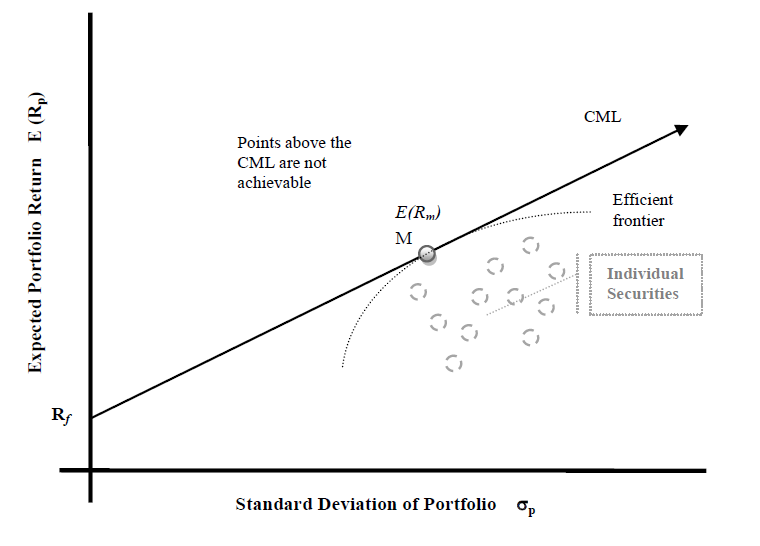
\includegraphics[width=\textwidth]{images/CML.png}
    \end{figure}
    \item Using the \textit{same} equations as before, we can calculate the expected return and standard deviation of an investor lying on the CML;
    \item We find the same results, but they are now based on a real market portfolio.
    \item The expected return of a portfolio on the CML is:
    \[E(R_p) = w_1R_f + (1-w_1)E(R_m)\]
    \[\sigma_p = (1-w_1)\sigma_m\]
    \item By substitution, $E(R_p)$ can be expressed in terms of $\sigma_p$, and this yield the equation for the CML:
    \[E(R_p) = R_f + \frac{E(R_m)-R_f}{\sigma_m} \times \sigma_p\]
\end{itemize}
\section{Derivation of the CAPM}
\begin{itemize}
    \item We now assume that all investors have access to the same market portfolio on the CML;
    \item The market portfolio is an efficient portfolio and contains all risky assets in the conomy with optimal weights;
    \item Each investor holds an optimal portfolio of risk-free assets and market portfolio that reflects his risk attitude.
    \begin{itemize}
        \item Graphically:
        \begin{figure}[h]
            \centering
            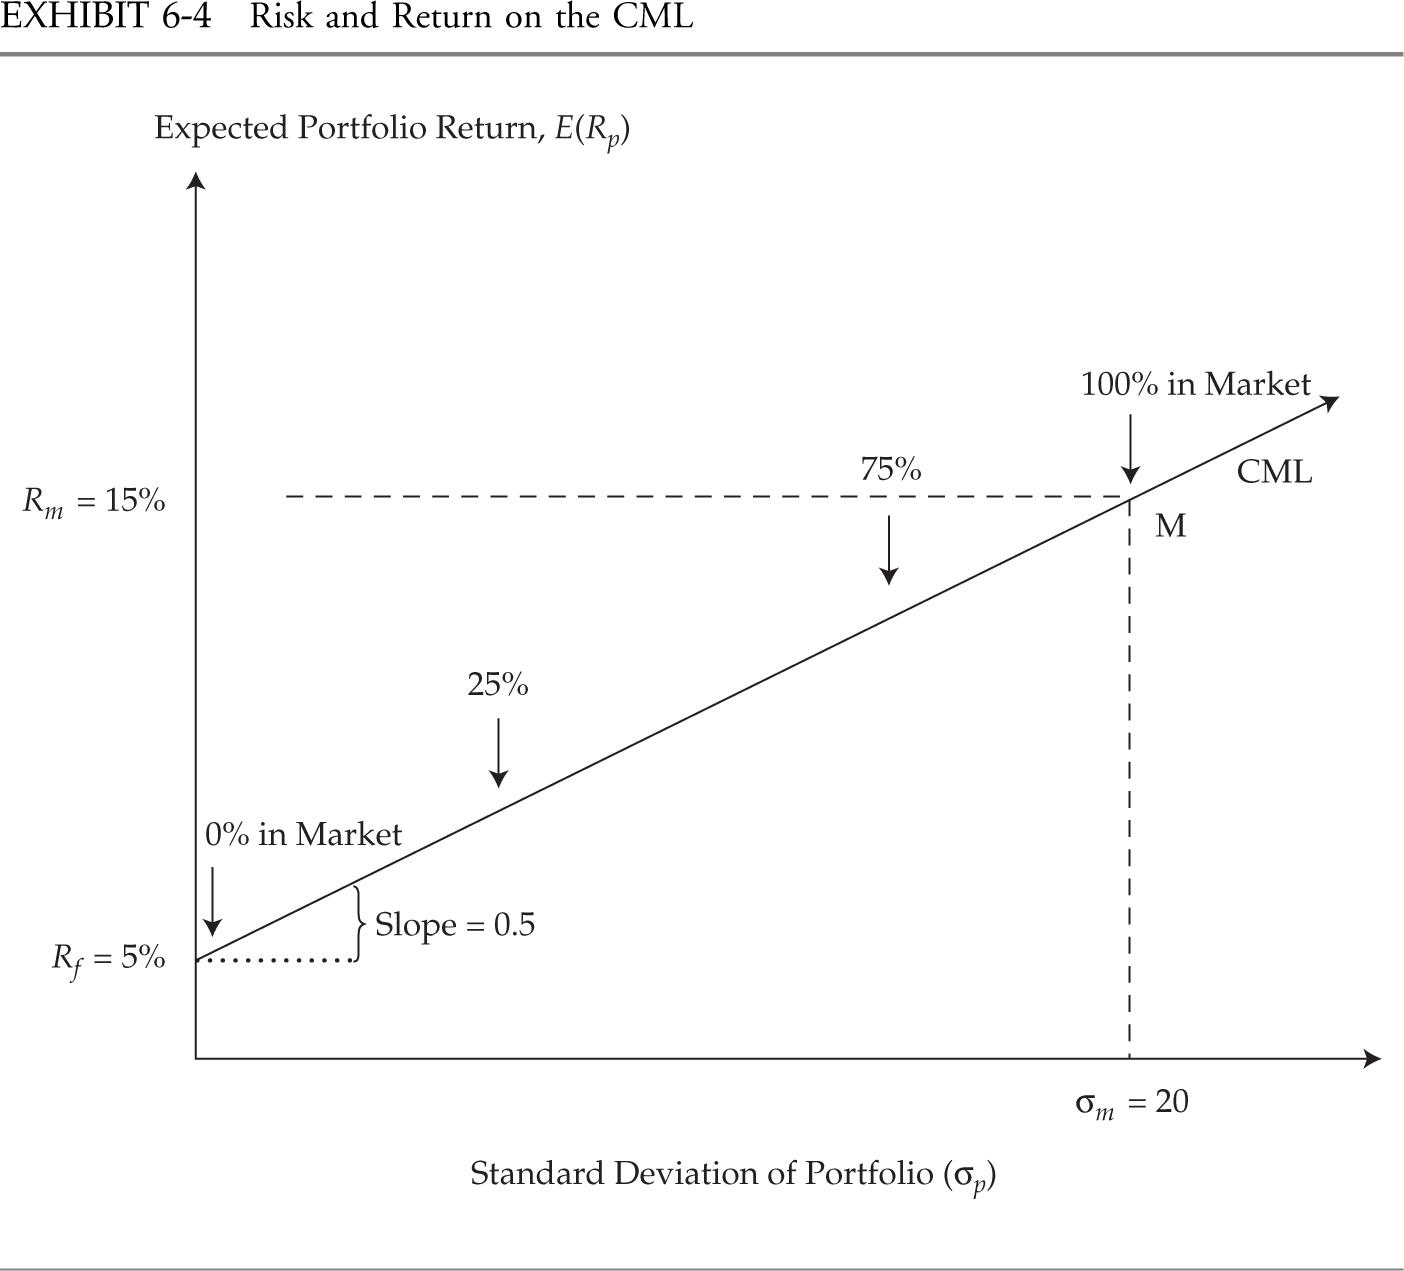
\includegraphics[width=\textwidth]{images/cml risk return.jpg}
        \end{figure}
    \end{itemize}
\end{itemize}
\subsection{Leveraged Portfolios}
An investor can go above 100\% in the market portfolio by borrowing. Meaning that there is a negative investiment in the risk-free asset. The lending and borrowing rate can be different.
\begin{figure}[h]
    \centering
    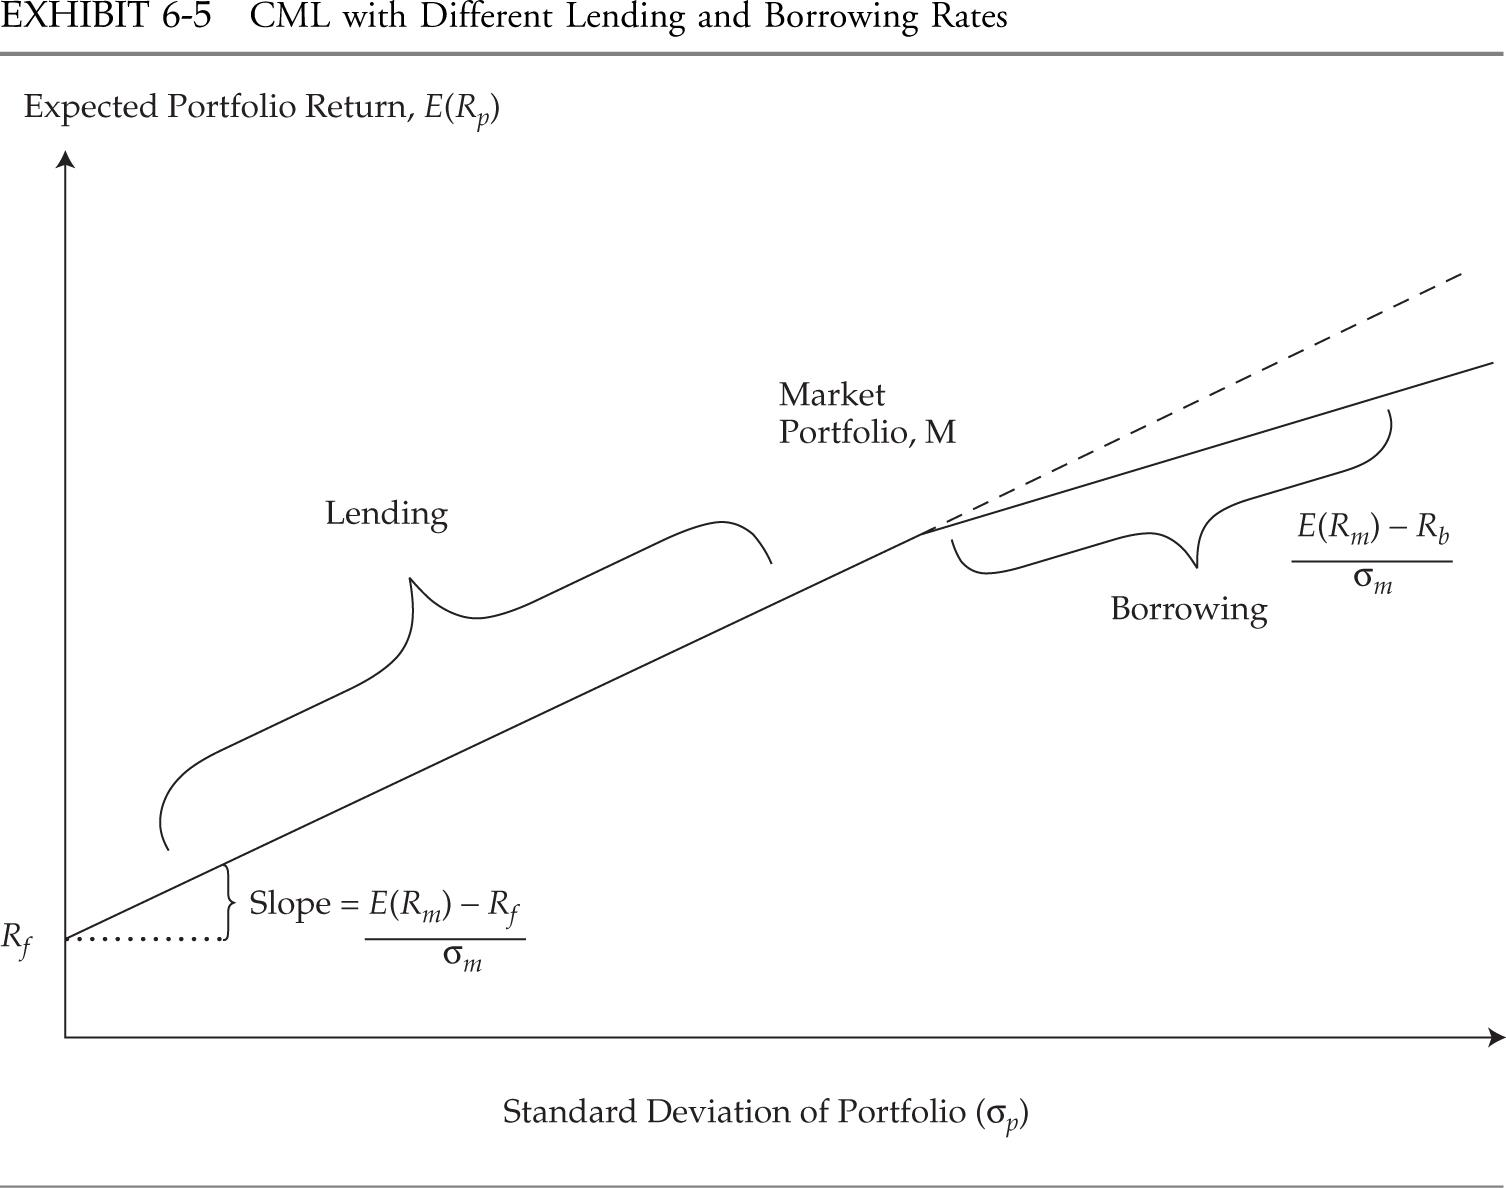
\includegraphics[width=\textwidth]{images/cml risk return w_borrowinglending.jpg}
\end{figure}
\subsection{Derivation of the CAPM}
\begin{itemize}
    \item Accessing the market portfolio means that we have included a very large number of securities;
    \item A portfolio's total risk can be categorized into two elemetens;
    \begin{itemize}
        \item Systematic Risk;
        \item Idiosyncratic Risk;
    \end{itemize}
\end{itemize}
\subsection{Portfolio of Many Risky Assets}
\begin{itemize}
    \item As long as we introduce assets with a correlation $<1$ we reduce the portfolio's risk;
    \item To see the share of specific and systematic risk, we can rewrite the variance equation of an equally-weighted protfolio, such as:
    \[\sigma_{p^2} = \sum_{i=1}^{n} w_{i^2}\sigma_{i^2} + \sum_{i, j=1, i \neq j}^{n} w_iw_jCov(i,j)\]
    \item As $n$ becomes larger, the first term on the right side, becomes smaller and smaller;
    \begin{itemize}
        \item The contribution of one asset's variance to the portfolio variance gradually becomes negligible.
    \end{itemize}
    \item The second term, however, approaches the average covariance as $n$ increases.
    \item For portfolios with a alrge number of assets, covariance among the assets accounts for almost all of the portfolio risk;
    \begin{itemize}
        \item Only the market, or \textbf{systematic} risk, remains.
    \end{itemize}
\end{itemize}
The access to the market protfolio menas that:
\begin{itemize}
    \item all non-systematic risk is diversified and they only endorse the systematic risk;
    \begin{itemize}
        \item Systematic risk = market risk;
        \item Idiosyncratic or specific risk = the security risk;
    \end{itemize}
    \item In finance, you are only paid for the risk you take;
    \begin{itemize}
        \item Investors are compensated only for systematic risk.
    \end{itemize}
\end{itemize}
\subsection{Derivation of the CAPM}
\begin{itemize}
    \item What if an asset would yield more than its sensitivity to the systematic risk?
    \item From the CAPM perspective, all investors hold the market portfolio, therefore are not affected by that specific risk;
    \item Investors can have return by holding non-diversified portfolios;
    \begin{itemize}
        \item However, total risk of the portfolio will increase.
    \end{itemize}
    \item As the diversification is a matter of investors' choice, the portfolio should be assessed by their sensibility to systematic risk;
    \begin{itemize}
        \item How much they move with the market - called \textbf{beta}.
    \end{itemize}
    \item Flip side: any investor should hold the optimal portfolio;
    \begin{itemize}
        \item Otherwise, they are exposed to the specific risk;
        \item Investors \textbf{must} diversify their portfolio to get a fair return.
    \end{itemize}
    \item So, we now know that an asset only yield its \textbf{sensitivity to the market risk};
    \item This is its \textbf{beta}: $\beta_i$
    \item The CAPM derives the formula of the beta.
    \item To estimate the price of an additional securirty, we should know how this secuirty modifies the risk of the portfolio \textbf{P};
    \item When a bit more of an asset \textit{x} is added to the market portfolio, investors only care how much risk asset \textit{x} adds to the risk of the market portfolio.
    \begin{itemize}
        \item Investors care about the change in the variance of the whole portfolio rather than individual variance.
    \end{itemize}
    \item The contribution of an asset to the riskiness of the market portfolio, is the new measure of riskiness for each component of an efficient portfolio.
    \item The risk premium on an asset will be determined by its contribution to the risk of investors' overall portfolios;
    \item For any individual asset \textit{x}, we can calculate the reward-to-risk ratio:
    \[\frac{E(r_x)-r_f}{\sigma_{x,M}}\]
    \item The numerator is the contribution of asset \textit{x} to the expected risk premium of the market portfolio.
    \begin{itemize}
        \item It measures the amount of risk increased y adding an asset.
    \end{itemize}
    \item The denominator is the contribution of asset \textit{x} to the risk of the market portfolio.
    \begin{itemize}
        \item There is no idiosyncratic risk.
    \end{itemize}
    \item For the market portfolio, we have:
    \[\frac{E(r_M)-r_f}{\sigma_{M^2}}\]
    \item This specific ratio is known as the market price of risk;
    \begin{itemize}
        \item Numerator - market risk premium;
        \item Denominator - risk of the market;
    \end{itemize}
    \item The ratio shows amount of market risk premium at the market risk level;
    \begin{itemize}
        \item It scales the net return of the portfolio by its risk.
    \end{itemize}
    \item At equilibrium, all assets must offer the same risk-return trade-off;
    \item This reflects the market price of risk - constant across securities;
    \item Re-writing the equation for any security \textit{x}:
    \[E(R_x) = r_f + \frac{\sigma_{x,M}}{\sigma_{M^2}}\times(E(r_M)- r_f)\]
    \item This gives us the expected return of the security \textit{x};
    \item It depends on \textbf{three elements}:
    \begin{itemize}
        \item The level of risk-free rate;
        \item The covariance of the asset \textit{x} with the market, scaled by the overall market variance: \textbf{sensibility to market risk};
        \item The expected return of the market portfolio (net of the risk-free rate);
    \end{itemize}
    \item It does \textbf{not} depend on the security's own risk.
\end{itemize}
\section{Calculation and Interpretation of the Beta}
\begin{itemize}
    \item Beta is the sensitivity to market risk;
    \begin{itemize}
        \item It is the second term of the equation as is calculated as:
        \[\beta_i = \frac{Cov(R_i,R_m)}{\sigma_{m^2}}\]
    \end{itemize}
    \item It captures an assets' systematic risk, or the portion of an asset risk that cannot be eliminated by diversification;
    \begin{itemize}
        \item The formula of the beta directly stems from portfolio theory - thus its hypotheses.
    \end{itemize}
    \item Everything else being constant (market return, market variance and risk-free rate), the return of a security only depends on its \textbf{covariance} with the market portfolio;
    \item The variance of an asset \textit{x} does not enter the expected return formula;
    \item This demonstrates that \textbf{only systematic risk} matters.
    \item As variance is always positive, we can easily interpret the \textbf{sign}of the beta;
    \item A \textbf{positive} beta indicates that the return of an asset follows the general market trend;
    \item A \textbf{negative} beta shows that the return of an asset generally follows a trend that is opposite to the market.
    \item Rewriting the beta in terms of correlation, we can deepen its interpretation;
    \item The beta is the correlation multiplied by the ratio of the security and the market volatitlity;
    \item It is not the sole correlation;
    \item All things being equal, the higher the correlation, the more $\beta$ tends to 1.
    \item A risk-free asset beta is zero;
    \item The beta of the market is one;
    \begin{itemize}
        \item The average beta of stocks in the market is also one;
    \end{itemize}
    \item Beta is not bounded;
    \item Even if a stock has a weak correlation with the market, if its volatility is high, compared to the market, the beta will be high;
    \item The sign of the beta, does not predict the sign of the return;
    \begin{itemize}
        \item Even with a negative beta, both the market and the asset can have positive returns;
    \end{itemize}
    \item A beta $< - 1$ means that the asset moves in an opposite direction \textbf{and} in a greater way than the market index;
    \item A beta between $-1$ and $0$ means that the asset moves in an opposite direction, \textbf{but} in a lesser way than the market;
    \item A beta between $0$ and $1$ means that the asset moves in the same direction, \textbf{but} in a less extent than the market;
    \item Beta $>1$ means that the asset moves in the same direction \textbf{and} in a greater way than the market;
    \item \textbf{Conclusion} - The CAPM shows that the primary determinant of expected return for a security is its beta or systematic risk.
    \item The CAPM is one of the most significant innovations in portfolio theory;
    \item The model is simple, yet powerful; intuitive, yet profound; and uses only one factor, yet is broadly applicable;
    \item It resolves the fundamental question of the cost of equity;
\end{itemize}
\section{The Security Market Line}
We can represent the equation of the CAPM graphically.
\[E(R_i) = R_f + \beta_i[E(R_m)-Rf]\]
\begin{itemize}
    \item This is called the secuirty market line (SML):
    \begin{itemize}
        \item Beta on the x-axis;
        \item Expected return on the y-axis;
        \item Rf is the y-intercept;
    \end{itemize}
    This line represents the relation between the expected return and the beta of an asset.
    \begin{figure}[h]
        \centering
        \includegraphics[width=\textwidth]{images/sml.png}
    \end{figure}
\end{itemize}
\section{Portfolio Beta}
It can be calculated from the expected return equation.
\begin{itemize}
    \item Portfolio beta is the weighted sum of the betas of the component secuirties:
    \item \[ \beta_p = \sum_{i=1}^{N}W_i\beta_i \]
    \item The portfolio's expected return is given by the CAPM;
    \item The return of any portfolio is now easily computable;
\end{itemize}
\section{Application of the CAPM}
\begin{itemize}
    \item The CAPM is used extensively in practice;
    \item There are three main applications:
    \begin{itemize}
        \item To give an estimate of expected return;
        \item To evaluate the performance of a portfolio;
        \item To select securities. 
    \end{itemize}
\end{itemize}
\subsection{Estimate of Expected Return}
\begin{itemize}
    \item The price of an asset is the sum of all the future cash-flows, discounted at the required rate of return;
    \item The CAPM provides an estimate of the required rate of return;
    \item For instance, for the FCF model
    \item \[V_0 = \sum_{t=1}^{\infty}\frac{CF_t}{(1+r)^t}\]
\end{itemize}
\subsection{Portfolio Performance Evaluation}
\begin{itemize}
    \item How to evaluate the performance of a portfolio (manager)?
    \item Active management is more costly: does it yield a better perfomance?
    \item Four ratios related to the CAPM are generally used in performance evaluation.
\end{itemize}
\subsubsection{Sharpe Ratio}
Sharpe Ratio focuses on total risk:
\[\frac{R_p - R_f}{\sigma_p}\]
\begin{itemize}
    \item It scales the excess return of the portfolio on its standard deviation;
    \item How much premium extracted for the risk taken;
    \begin{itemize}
        \item The higher, the better!
    \end{itemize}
\end{itemize}
\subsubsection{M-Squared}
$M^2$ is an extension of the Sharpe ratio:
\[ (R_p - R_f) \frac{\sigma_m}{\sigma_p} - (R_m - R_f) \]
\begin{itemize}
    \item $M^2$ gives rankings that are identical to those of the Sharpe ratio;
    \item A portfolio that matches the performance of the market will have an $M^2$ of zero, whereas a portfolio that outperforms the market will have an $M^2$ that is positive;
    \item They are easier to interpret, however, because they are in percentage terms;
    \item We can see whether the portfolio beats the market on a risk-adjusted basis.
\end{itemize}
\subsubsection{Treynor Ratio}
The Tryenor ratio draws on the CAPM beta:
\[\frac{R_p - R_f}{\beta_p}\]
\begin{itemize}
    \item It gives the excess return (risk premium), scaled by the systematic risk taken;
    \item The idea is that only the systematic risk should be taken into account, as idiosyncratic risk is already diversified.
\end{itemize}
\subsubsection{Jensen's Alpha}
\begin{itemize}
    \item Jensen's alpha also draws on the CAPM beta;
    \item It gives the excess return obtained with this portoflio, that is not predicted by the CAPM.
    \[\alpha_p = R_p - E[R_p]\]
    \[\alpha_p = R_p - [R_f + \beta_p(R_m - R_f)]\]
    \item "Abnormal return" - can be attributed to the performance of the manager.
    \item Jensen's alpha can be represented graphically:
    \[R_i - R_f = \alpha_i + \beta_i(R_m - R_f)\]
    \item This is called the \textbf{Security Characteristic Line (SCL)}
    \begin{itemize}
        \item On the y-axis: the security excess return;
        \item On the x-axis: the market excess return.
    \end{itemize}
    \item Alpha is the y-intercept and beta the slope;
    \item While the SML is for the market portfolio, the SCL gives the relative performance of a portfolio.
    \begin{figure}[h]
        \centering
        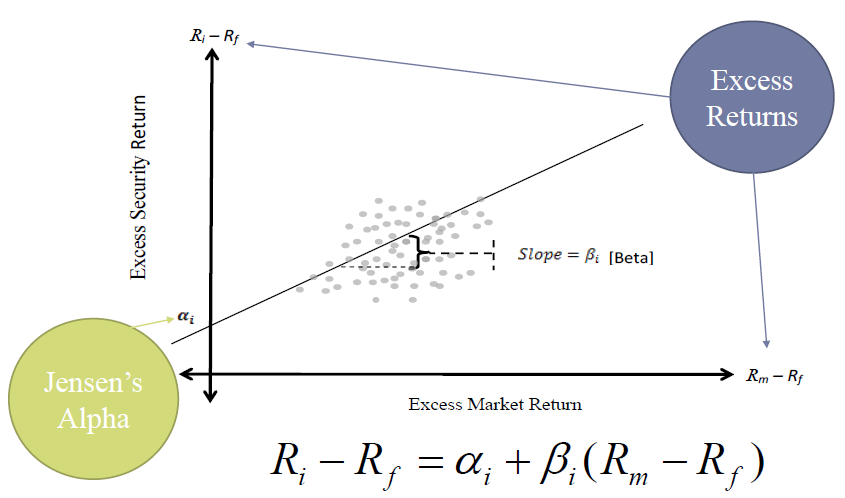
\includegraphics[width=\textwidth]{images/SCL.png}
    \end{figure}
\end{itemize}
\subsubsection{Measures of Portfolio Performance}
\begin{itemize}
    \item We now have 4 measures of portfolio performance;
    \item Two of them draw on the total risk, while two draw on the portfolio beta;
    \item They offer different perspectives on the performance of a fund:
    \begin{itemize}
        \item They are useful to synthesise different infromation.
    \end{itemize}
\end{itemize}
\subsection{Security Selection}
\begin{itemize}
    \item When we built the CAPM, we assume that investors hold common beliefs and expectations;
    \item Here, we introduce heterogeneity in beliefs of investors;
    \begin{itemize}
        \item Tehy do not have similar expectations.
    \end{itemize}
    \item Investors are price-takers, it is assumed, that such heterogeneity does not significantly affect the market price of an asset;
    \item Differences in beliefs could result in an \textbf{investor-estimated} return that is different from the CAPM calculated return;
    \item Jensen's alpha can be used for security selection.
    \item If alpha is different from zero, it means that there is a residual (positive or negative) return which is not priced in the security by the CAPM;
    \item This is due to different expectations between the investor and the overall market.
    \item From this perspective, an investor shoud:
    \begin{itemize}
        \item \textbf{Buy} an asset with a positive alpha, because it is undervalued;
        \item \textbf{Sell} an asset with a negative alpha, because it is overvalued.
    \end{itemize}
    \item This is done using the \textbf{Security Market Line};
    \item Investors can then plot their own expectations on the SML graph:
    \begin{itemize}
        \item Above the SML - higher returns for the same $\beta$ - undervalued (\textbf{buy})
        \item Below the SML - lower returns for the same $\beta$ - overvalued (\textbf{sell})
    \end{itemize}
    \begin{figure}[h]
        \centering
        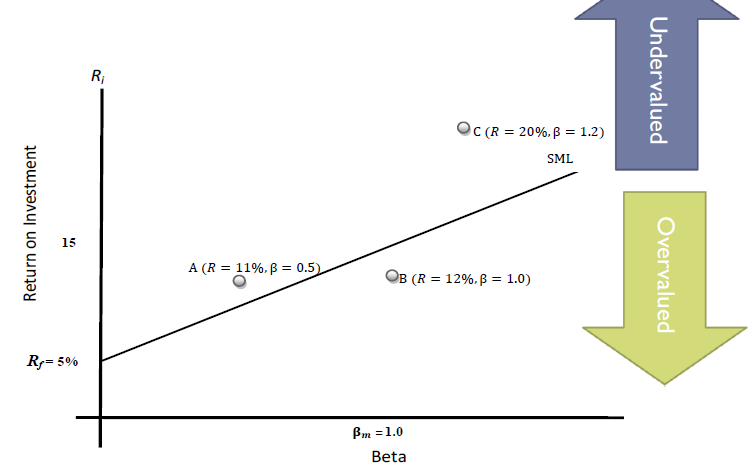
\includegraphics[width=\textwidth]{images/security selection.png}
    \end{figure}
\end{itemize}
\subsection{Constructing a Portfolio}
\begin{itemize}
    \item The more practical way to start is to hold a broad protfolio security;
    \begin{itemize}
        \item The S\&P500 is available for trade and offers the largest US corporations.
    \end{itemize}
    \item Any security not included in the S\&P500 can be evaluated to determine whether it should be included.
    \item To make the decision, one computes the alpha of the security.
    \item A security with a positive alpha means additional returns in comparison with the market portfolio - should be included.
    \begin{itemize}
        \item A security with a negative $\alpha$ can be short sold.
    \end{itemize}
    \item Similarly, one can compute the alpha of the securities within the S\&P500 and decide which to keep;
    \item If $\alpha$ indicates higher returns compared to the market portfolio, which wheight should be given to the security?
    \item We aim to maximize \textbf{risk-adjusted returns}:
    \begin{itemize}
        \item Securities with a higher alpha should have a higher weight;
        \item Securities with greater nonsystematic risk should be given less weight in the portfolio.
    \end{itemize}
    \item The information ratio:
    \[\frac{R_i - E(R_i) = \alpha_i}{\sigma_{\alpha_i}}\]
    \item It measures the abnormal return per unit of risk (risk-adjusted returns) added by the security to a well-diversified portfolio;
    \item The larger the information rato is, the more valuable is the security to be in the portfolio.
\end{itemize}
\section{Beyond the CAPM}
\subsection{Limitations of the CAPM}
The CAPM is a powerful tool to estimate an expected return for any asset. However it has its limits:
\begin{itemize}
    \item Underlying assumptions;
    \item Theoretical limitations;
    \item Practical limitations;
    \item We can identify 8.
\end{itemize}
\subsubsection{Single-factor model}
\begin{itemize}
    \item Only systematic risk or beta risk is priced in the CAPM;
    \item Thus, the CAPM states that no other investment characteristics should be considered in estimating returns;
    \item As a consequence, it is prescriptive and easy to understand and apply, although it is very restrictive and inflexible.
\end{itemize}
\subsubsection{Single-period model}
\begin{itemize}
    \item The CAPM does not consider multi-period implications or investment objectives of future periods, which can lead to myopic and suboptimal investment decisiions;
    \item The only horizon is the one of expected returns;
    \item A single-period model like the CAPM is unable to capture factors that vary over time adn span several periods.
\end{itemize}
\subsubsection{Homogeneity in investor expectations}
\begin{itemize}
    \item The CAPM assumes that homogeneity exists in investor expectations for the model to generate a single optimal risky portfolio (the market) and a single securirty market line;
    \item Without this assumption, there will be numerous risky portfolios and numerous security market lines;
    \item Clearly, investors can process the same information in a rational manner and arrive at different optimal risky portfolios. This is assumed in secuirty selection.
\end{itemize}
\subsubsection{Market portfolio}
\begin{itemize}
    \item The true market portfolio according to the CAPM includes all assets, financial and non-financial, which means that it also includes many assets that are not investable, such as human capital and assets in closed economies;
    \item Richard Roll noted that one reason the CAPM is not testable is that true market portfolio is unobservable.
\end{itemize}
\subsubsection{Proxy for a market portfolio}
\begin{itemize}
    \item In the absence of a true market portfolio, market participants generally use proxies;
    \item These proxies, however, vary among analysts, the country of the investor - and so on - generating different return estimates for the same asset, which is impermissible in the CAPM;
\end{itemize}
\subsubsection{Estimation of beta risk}
\begin{itemize}
    \item There is no consensus on the length of the estimation period;
    \item Using different periods for estimation results in different estimates of beta;
    \item Companies may not have enough historical data;
    \item Thus, we are likely to estimate different returns for the same asset, depending on the estimate of beta risk used in the model.
\end{itemize}
\subsubsection{Efficient Markets}
\begin{itemize}
    \item Observed returns lies on the assumption that markets are efficient - investors possess all the information and the means to trade assets:
    \begin{itemize}
        \item Cost efficiency;
        \item Information efficiency;
        \item Allocation efficiency.
    \end{itemize}
    \item This is rarely the case, and there are different levels of market efficiency;
    \item This impacts the expected return and CAPM predictions.
\end{itemize}
\subsubsection{Normal Distribution}
\begin{itemize}
    \item The portfolio approach relies on a mean-variance analysis, makign the assumption that returns are normally distributed;
    \item Using only mean and variance would be appropriate to evaluate instruments if returns were normally distributed;
    \item However, returns are not normally distributed. They are:
    \begin{itemize}
        \item Skewed: they are not symmetric around the mean;
        \item Characterized by a high probability of extreme events.
    \end{itemize}
\end{itemize}
\subsection{Limitations of the CAPM}
Overall, these limitations make the CAPM a poor predictor of returns:
\begin{itemize}
    \item If the CAPM is a good model, its estimate of asset returns should be closely associated with realized returns;
    \item However, empirical support for the CAPM is weak. In other workds, tests of the APM show that asset returns are not determined only by systematic risk;
    \item Poor predicatability of returns when using the CAPM is a serious limitation because return-generating models are used to estimate future returns.
\end{itemize}
\subsection{Extensions of the CAPM}
New models have been suggested to overcome the limitations of the CAPM, creating their own limitations.
\subsubsection{X-Factors CAPM}
\begin{itemize}
    \item Historical analysis shows that the coefficient on market return is not significantly different from zero, which implies that sotck returns are unrelated to the market.
    \item In 1992, Fama and French offer a three factor model:
    \begin{itemize}
        \item size (smaller companies outperform larger companies) - Small-Minus-Big;
        \item Book-to-Market ratio (value companies with low BM ratio outperform glamour companies) - High-Minus-low.
    \end{itemize}
    \item In 1997, Carhart add a momentum factors:
    \begin{itemize}
        \item Momentum (past winners outperform past losers) - Winner-Minus-Losers.
    \end{itemize}
\end{itemize}
\subsubsection{X-Factor Models}
\begin{itemize}
    \item The underlying concept behind the model is that the return generated by portfolio managers are due in part to factors that are beyond the managers' control;
    \item Specifically, value stock have historically outperformed growth stock on average, while smaller companies have outperformed larger ones;
    \item These factors are at the market-level - each stock will have a specific sensitivity to it.
\end{itemize}
\subsubsection{3-Factors CAPM}
You then obtain "factors":
\begin{itemize}
    \item These are numerical values;
    \item They are at the market-level;
    \item People use the values provided by Fama and French.
    \[E(R_{it} - R_f = \alpha_i + \beta_{i,MKT}MKT_t + \beta{i,SMB} SMB_t + \beta{i,,HML} HML_t)\] , MKT = Systematic Risk, SMB = Size Anomaly, HML = Value Anomaly;
    \item You then employ an OLS-regression to esmitate the sinsibility of a given secuirty to the market wide factor.
\end{itemize}
\subsubsection{4-Factors CAPM}
    \begin{itemize}
    \item There is an improvement in the R-square compared with the one-factor model;
    \[E(R_{it} - R_f = \alpha_i + \beta_{i,MKT}MKT_t + \beta{i,SMB} SMB_t + \beta{i,,HML} HML_t + \beta_{i,WML}WML_t)\] , MKT = Systematic Risk, SMB = Size Anomaly, HML = Value Anomaly, WML = Momentum Anomaly
    \end{itemize}
\subsubsection{Practical Models}
\begin{itemize}
    \item The three and four-factor models have been found to predict asset returns much better than the CAPM:
    \begin{itemize}
        \item It is extensively used in estimating returns for U.S stocks;
    \end{itemize}
    \item Recent work expand the number of factors:
    \begin{itemize}
        \item In 2015 Fama and French offer a five factor model;
        \item They add profitability and investment.
    \end{itemize}
\end{itemize}
\subsubsection{Factor Models}
\begin{itemize}
    \item Factor models try to estimate the expected returns based on a list of variables;
    \item The best example is the \textbf{Arbitrage Pricing Theory (APT)};
    \item Like the CAPM, APT proposes a linear relationship between expected return and risk;
    \item It can include many factors, without considering theoretical framework of the CAPM.
\end{itemize}
\subsubsection{APT Model}
\begin{itemize}
    \item The APT model does not make specific assumptions like the CAPM;
    \item The market can misprice an asset, and arbitrageurs can take the opportunity to make profits;
    \item Which factors to use is really dependent on empirical research, and the investor's gut.
    \[E(R_p) = R_F + \lambda_1\beta_{p,1} + ... + \lambda_K\beta_{p,K}\], $\lambda$ = Risk Premium for Factor 1, $\beta_{p,1}$ = Sensitivity of the Portfolio to Factor 1
    \item Unlike the CAPM, APT allows for numerous risk factors (K) - as many as relevant to a particular asset;
    \item Other than the risk-free rate, the risk factors do not need to be common and may vary from one asset to antoher;
    \item The coefficient of each factor is estimated using econometric models;
    \item Common factors are GDP growth, inflation, M3 growth, S\&P return, VIX, etc;
    \item APT is not often used, because it is more time-consuming to implement;
    \item Though, it can be developed internally to offer a valuation tool to traders;
    \item It does rely a lot on the decision to include certain factors, but modern big data approaches can allow to better select them, and outperform the CAPM.
\end{itemize}
\chapter{Behavioural Finance - Portfolio Management Industry}
\section{Efficient Market Hypothesis}
\begin{itemize}
    \item There are many investors out there doing market analysis;
    \item If investors are not analysing the stcok price, the market wouldn't be efficient;
    \item An efficient market means that you will earn a return that is appropriate for the risk undertaken and that there are no bias to be exploited to eran an excess return;
    \item Market efficiency will not protect you from wrong choices, if you do not diversify.
\end{itemize}
\subsection{Forms of Market Efficiency}
\begin{itemize}
    \item Weak Form Efficiency - prices reflect \textbf{\underline{all historical market information}} such as price and volume;
    \begin{itemize}
        \item Invesors cannot earn abnormal returns by trading on past market data.
    \end{itemize}
    \item Semi-strong Form Efficiency - prices reflect all \textbf{\underline{publicly available information}} including trading information, annual reports, press releases, etc;
    \begin{itemize}
        \item investors cannot earn abnormal returns by trading on public information.
    \end{itemize}
    \item Strong Form Efficiency - reflect \textbf{\underline{all information, including public and private}};
    \begin{itemize}
        \item investors could not earn abnormal returns regardless of the information they possessed.
    \end{itemize}
    \item Empirical evidence indicates that\textbf{\underline{markets are generally weka (or semi-strong) form efficient}}.
\end{itemize}
\subsection{What is Behavioural Finance?}
There are three sub fields to modern financial research.
\begin{itemize}
    \item \textit{Theoretical finance} is the study of logical relationships among assets;
    \item \textit{Empirical finance} deals with the study of data in order to infer relationships;
    \item \textit{Behavioural finance} integrates psychology into the investment process.
\end{itemize}
\begin{itemize}
    \item Behavioural finance research focuses on:
    \begin{itemize}
        \item how investors make decisions to buy and sell secuirties;
        \item how they choose between alternatives, and
        \item how \textbf{\underline{reasoning erors}} influence investor decisions and market prices.
    \end{itemize}
    \item Much of behavioural finance research stems from the research in the are of cognitive psychology;
    \item Some people believe that cognitive errors made by investors will cause market inefficiencies.
\end{itemize}
\section{Standard vs. Behavioural Finance}
\subsection{Standard Finance}
\begin{itemize}
    \item People are rational;
    \item People construct portfolios as described by mean-variance portfolio theory, where they want to include only high expected returns and low risk;
    \item People save and spend as described by standard life-cycle theory;
    \item Expected returns of investments are accounted for by standard asset pricing theory, where differences in expected returns are determined only by differences in risk;
    \item Markets are efficient, in the sense that prices equal values in them and in the sense that they are hard to beat;
\end{itemize}
\subsection{Behavioural Finance}
\begin{itemize}
    \item People are normal;
    \item People construct portfolios described by behavioural portfolio theory, where they want to extend beyond high expected returns and low risk, such as for social responsibility and social status;
    \item People save and spend as described by behavioural lifecycle theory, where impediments, such as weak self-control, make it difficult to find and follow the right way to save and spend;
    \item Expected returns of investments are accounted for by behavioural asset pricing theory, where different in expected returns are determined by more than differences in risk, such as by levels of social responsibility and social status;
    \item Markets are not efficient in the sense that prices equal values in them, but they are hard to beat.
\end{itemize}
\section{Prospect Theory}
\begin{itemize}
    \item Prospect theory provides an alternative to classical, rational economic decision-making;
    \item Risk averse investors get increasing utility from higher levels of wealth, but at a decreasing rate;
    \item Research shows that while risk aversion may accurately describe investor behaviour with gains, investors often show risk seeking behaviour when they face a loss;
    \item The foundation of prospect theory: investors are much more distressed by prospective losses than they are happy about prospective gains.
    \item \begin{figure}[h]
        \centering
        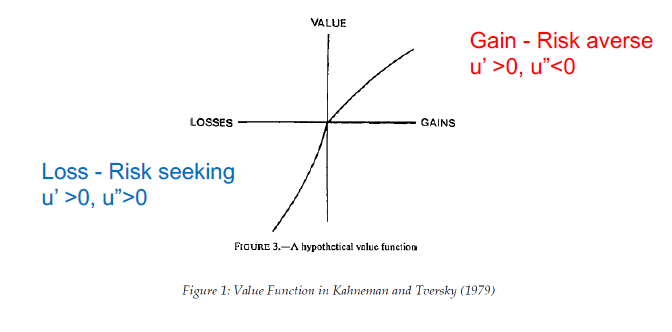
\includegraphics[width=\textwidth]{images/prospect theroy.png}
    \end{figure}
    \item There are well-know judgement errors consistent with the predictions of prospect theory.
    \begin{itemize}
        \item Frame dependence - tendency that people make decision depends on how situation is framed;
        \item Mental accounting - tendency to put things in different imaginary account;
        \item The House Money effect - willing to take big risks with money wom from gambling;
    \end{itemize}
\end{itemize}
    \subsection{Frame Dependence}
    If an investment problem is presented in two different ways (with identical results), investors often make inconsistent choices.
    \subsection{Mental Accounting}
    \begin{itemize}
        \item Mental accounting refers to our tendency to "put things in boxes" and track them individually;
        \item Transaction utility;
        \begin{itemize}
            \item The perceived value of the "deal" - difference between amount paid and reference price;
        \end{itemize}
        \item Opening and closing accounts;
        \begin{itemize}
            \item Realized vs. paper gain (or loss);
            \item Realized gain (or loss) is more delightful (painful);
            \item Mental accounting favours selling the winner;
        \end{itemize}
        \item Advance purchase, sunk costs and payment depreciation;
        \item Payment decoupling;
        \begin{itemize}
            \item Credit card: later payment \& installment;
        \end{itemize}
    \end{itemize}
    \subsubsection{Choice Bracketing and Dynamic Mental Accounting}
    \begin{itemize}
        \item Narrow framing and myopic loss aversion;
        \begin{itemize}
            \item Loss-averse people are willing to take risk if they combine many bets together;
        \end{itemize}
        \item Diversification heuristic
        \begin{itemize}
            \item Variety-seeking: people tend to diversify, when they are asked to make several choices at once.
        \end{itemize}
    \end{itemize}
    \subsection{The House Money Effect}
    \begin{itemize}
        \item Thinking this way means that you are guilty of playing with house money;
        \item Whether you lose money from your original investment (your money) or lose money from your investment gains (house money) is irrelevant;
        \item There are two important investment lessons:
        \begin{itemize}
            \item There are no "paper profits". Your profits are yours;
            \item All your money is your money. You should not separate your money into bundles labelled "my money" and "house money".
        \end{itemize}
    \end{itemize}
\section{Overconfidence}
\begin{itemize}
    \item A serious error in judgement you can make as an investor is to be overconfident;
    \item We are all overconfident about our abilities in many areas.
\end{itemize}
\subsection{Overconfidence and Portfolio Diversification}
\begin{itemize}
    \item Investors tend to invest too heavily in shares of the company for which tehy work;
    \item This loyalty can be very bad financially:
    \begin{itemize}
        \item Your earning power (income) depends on this company;
        \item Your retirement nest-egg also depends on this company.
    \end{itemize}
    \item Another example of the lack of diversification is investing too heavily in the stocks of local companies:
    \begin{itemize}
        \item Perhaps you know someone personally who works there;
        \item Perhaps you read about them in your local paper;
        \item Basically, you are unduly confident that you have a high degree of knowledge about local companies.
    \end{itemize}
\end{itemize}
\subsection{Overconfidence and Trading Frequency}
\begin{itemize}
    \item If you are overconfident about your investment skill, it is likely that you will trade too much;
    \item Researchers have found that investors who make relatively more trades havelower returns than investors who trade less frequently;
    \item The moral is clear: \textbf{Excessive trading is hazardous to your wealth}.
    \item Psychologists have found that mean are more overconfident than women in the area of finance.
    \item Men trade about 45\% more than women;
    \item Accounting for the effects of marital status, age and income, researchers also show that men invest in riskier positions.
\end{itemize}
\section{Regret Avoidance}
\begin{itemize}
    \item Did I screw up or am I just unlucky?
    \item "Courageous" to invest in these firms. I need a bigger return. I will discount the cashflows of these firms at a higher rate. The price is lower and my reutrn is higher.
\end{itemize}
\section{Herd Behaviour}
\begin{itemize}
    \item A phenomenon in which individuals act collectively as a group;
    \item Often, individual investors mimic the actions of a larger group or markt, rather thean following their own analysis;
    \item This happens when there is: lack of experience, social pressure;
    \item Herd behaviour is a significant driver of extreme volaility and asset bubbles in financial markets - e.g. 2008 financial crisis, bitcoin bubble, etc;
\end{itemize}
\section{Emotional Gap}
\begin{itemize}
    \item Refers to decision making based on extreme emotions or emotional strains such as anxiety, anger, fear or excitement;
\end{itemize}
\section{Anchoring}
\begin{itemize}
    \item Bias that a certain price they choose for some reason would work as an individual is given a pice of information to which they refer subsequent judgements during decision making.
    \begin{itemize}
        \item Market anomalies/inefficiencies and Technical analysis (support/resistance) can be explained by anchoring;
        \item Investors are slow to adjust their expectations to the present price;
    \end{itemize}
\end{itemize}
\section{Self-attribution}
\begin{itemize}
    \item Self-attribtion bias: individuals' tendency to attribute successes to personal skills and failures to factors beyond their control;
    \begin{itemize}
        \item Individuals tend to overlook their mistakes or external factors;
    \end{itemize}
\end{itemize}
\section{Culture and Investment Behaviour}
\begin{itemize}
    \item Cultural differences matter for financial decisions;
    \item Cultural differences lead to systematic deviations from rational decision making in:
    \begin{itemize}
        \item risk taking;
        \item negotiations for direct investment, mergers \& acquistions;
        \item returns of bonds and stocks at local markets;
    \end{itemize}
\end{itemize}
\section{Application of Behavioural Finance - Technical Analysis}
\begin{itemize}
    \item \textbf{Technical analysis} attempts to exploit \textbf{recurring and predictable patterns in stock prices} to generate superior investment performance;
    \item This is different from the \textbf{fundamental analysis} which attempts to measure \textbf{the security's intrinsic value by reviewing financial and non-financial factors};
    \item Technicians do not deny the value of fundamental information. But they believe that prices only gradually close in on intrinsic value;
\end{itemize}

\end{document}